\documentclass[11pt]{article}
\usepackage[utf8]{inputenc}
\usepackage[T1]{fontenc}
\usepackage[french]{babel}
\usepackage{amsmath}
\usepackage{graphicx}
\usepackage[margin=1in]{geometry}
\usepackage{enumitem}
\usepackage{listings}
\usepackage{xcolor}
\lstdefinelanguage{OCaml}{
  morekeywords={let, in, rec, match, with, type, module, struct, fun, function, val, open, and, if, then, else, begin, end},
  sensitive=true,
  morecomment=[s]{(*}{*)},
  morestring=[b]",
}
\usepackage{xcolor}
\usepackage{caption}

\title{
  Data Test : BIFORA
}
\author{
  ROBERT Wendy
}
\date{\today}
\lstset{
  basicstyle=\ttfamily\small,
  keywordstyle=\color{blue},
  commentstyle=\color{gray},
  stringstyle=\color{orange},
  breaklines=true,
  frame=single,
  captionpos=b,
  showstringspaces=false,
  language=OCaml
}
\begin{document}

\maketitle
\tableofcontents
\newpage

\section*{Introduction}
L'objectif de ce travail est d'analyser et de préparer un jeu de données issu d'un fichier Excel fourni. 
Ce fichier comporte deux feuilles principales (\texttt{Data\_1} et \texttt{Data\_2}) décrivant des informations 
sur une base de clients, ainsi qu'une troisième feuille (\texttt{TYPES VARIABLES}) servant de dictionnaire de données. 

% --- import ---
\section{Traitement}

\subsection{Python}

L'analyse débute par l'importation du fichier Excel \texttt{data\_test\_BIFORA.xlsx} contenant trois feuilles de données : 
\texttt{Data\_1}, \texttt{Data\_2} et \texttt{TYPES VARIABLES}. 
Cette opération est réalisée en Python grâce à la bibliothèque \texttt{pandas}, qui permet de lire directement des fichiers Excel.

\subsubsection{Chargement des bibliothèques}
Nous commençons par importer la bibliothèque \texttt{pandas} :

\begin{lstlisting}[caption=Importation bibliothèque Pandas]
import pandas as pd
\end{lstlisting}


\subsubsection{Lecture du fichier Excel}
Ensuite, nous spécifions le chemin du fichier et chargeons les trois feuilles de données :

\begin{lstlisting}[caption=Importation du fichier Excel]
    # Importation des 3 feuilles
    path = r"/Users/wendyr/Downloads/data_test_BIFORA (2) (1).xlsx"
    data1 = pd.read_excel(path, sheet_name="Data_1")
    data2 = pd.read_excel(path, sheet_name="Data_2")
    dict_vars = pd.read_excel(path, sheet_name="TYPES VARIABLES ")
    \end{lstlisting}

Une fois les données importées, nous pouvons examiner leurs dimensions, leurs colonnes et les premières lignes afin de comprendre leur structure :


Cette étape constitue la base de toute l'analyse, car elle permet de vérifier que les données sont bien accessibles et lisibles par Python avant de passer au diagnostic et au nettoyage.
\subsubsection{Préparation et nettoyage des données}
Certaines variables contiennent des erreurs de frappe ou des espaces parasites dans leur nom. Nous commençons par corriger ces problèmes et nettoyer les colonnes :

\begin{lstlisting}[language=Python, caption=Renommage et nettoyage des colonnes]
# Renommer correctement la variable identifiant
data1 = data1.rename(columns={"identiffiant ": "identifiant"})

# Nettoyer les noms des variables (suppression des espaces)
data1.columns = data1.columns.str.strip()
data2.columns = data2.columns.str.strip()
dict_vars["VARIABLES"] = dict_vars["VARIABLES"].str.strip()
\end{lstlisting}
\subsubsection{Diagnostic initial des données}
Pour mieux comprendre la structure des jeux de données, nous définissons une fonction \texttt{diagnostic} qui affiche les types de variables, les valeurs manquantes et les doublons :

\begin{lstlisting}[language=Python, caption=Diagnostic des bases]
def diagnostic(df, name):
    print("\n--- Diagnostic "+name+" ---")
    print("Types de variables :\n", df.dtypes)
    print("\nValeurs manquantes :\n", df.isna().sum())
    print("\nDoublons :", df.duplicated().sum())

diagnostic(data1, "Data_1")
diagnostic(data2, "Data_2")
\end{lstlisting}

\subsubsection{Suppression des doublons et fusion des bases}
Nous supprimons les doublons et fusionnons les deux jeux de données sur la variable \texttt{identifiant} :

\begin{lstlisting}[language=Python, caption=Nettoyage et fusion des données]
data1 = data1.drop_duplicates()
data2 = data2.drop_duplicates()

merged = data1.merge(data2, on="identifiant", how="inner")

print("\nDimensions Data_1 :", data1.shape)
print("\nDimensions Data_2 :", data2.shape)
print("\nDimensions après fusion :", merged.shape)
\end{lstlisting}

\subsubsection{Renommage et sélection des variables pertinentes}
Pour harmoniser les noms de colonnes et conserver uniquement les variables nécessaires à l'analyse :

\begin{lstlisting}[language=Python, caption=Renommage et sélection des variables]
rename_map = {
    "AGE": "age",
    "SEXE": "sexe",
    "MARCHE": "marche",
    ...
}
merged = merged.rename(columns=rename_map)

needed = ["age", "marche", "csp", "type_client", "situation_famille", "epargne_financiere", "epargne_total"]
merged = merged[needed].copy()
\end{lstlisting}

\subsubsection{Conversion des variables en numérique}
À l'aide du dictionnaire \texttt{TYPES VARIABLES}, nous convertissons les variables quantitatives. Les erreurs de conversion sont transformées en \texttt{NaN} :

\begin{lstlisting}[language=Python, caption=Conversion numérique et suppression des valeurs manquantes]
for _, row in dict_vars.iterrows():
    var = row["VARIABLES"]
    if var in data1.columns and row["Quali / Quanti "] == "Quanti":
        data1[var] = pd.to_numeric(data1[var], errors="coerce")
    if var in data2.columns and row["Quali / Quanti "] == "Quanti":
        data2[var] = pd.to_numeric(data2[var], errors="coerce")

for col in ["age", "epargne_financiere", "epargne_total"]:
    if col in merged.columns:
        merged[col] = pd.to_numeric(merged[col], errors="coerce")

merged = merged.dropna(subset=["age", "epargne_total", "epargne_financiere"])
\end{lstlisting}

\subsection{SAS}

En parallèle de Python, les données ont également été importées dans SAS afin de permettre une exploration complémentaire et des traitements statistiques. 

\subsubsection{Définition de la librairie et importation}
Tout d'abord, une librairie pointant vers le fichier Excel a été définie. L'instruction \texttt{proc import} a ensuite été utilisée pour lire directement les feuilles \texttt{Data\_1} et \texttt{Data\_2} :

\begin{lstlisting}[caption=Importation des données dans SAS]
libname x xlsx '/home/u64300920/data_test_BIFORA (2) (1).xlsx';

/* Import feuille Data_1 */
proc import datafile='/home/u64300920/data_test_BIFORA (2) (1).xlsx'
    out=x.data1
    dbms=xlsx
    replace;
    sheet="Data_1";
    getnames=yes;
run;

/* Import feuille Data_2 */
proc import datafile='/home/u64300920/data_test_BIFORA (2) (1).xlsx'
    out=x.data2
    dbms=xlsx
    replace;
    sheet="Data_2";
    getnames=yes;
run;
\end{lstlisting}

\subsubsection{Conversion des variables mal typées}
Lors de l'importation, certaines variables continues (par exemple \texttt{Epargne\_financiere}) ont été interprétées comme du texte.  
Afin de pouvoir effectuer des analyses statistiques correctes, elles ont été converties en variables numériques à l'aide de la fonction \texttt{input()} :

\begin{lstlisting}[caption=Conversion de variables texte en numérique]
/* Création d'une nouvelle version de Data_1 avec conversion */
data x.data1_num;
    set x.data1;
    Epargne_financiere_num = input(Epargne_financiere, best32.);
    drop Epargne_financiere;
    rename Epargne_financiere_num = Epargne_financiere;
run;
\end{lstlisting}

Cette étape garantit que les montants financiers pourront être utilisés dans des calculs (sommes, moyennes, médianes, etc.).

\subsubsection{Contrôle de l'importation}
Enfin, une inspection des structures des tables a été réalisée avec la procédure \texttt{proc contents}, afin de vérifier la nature des variables importées (caractère ou numérique) :

\begin{lstlisting}[caption=Inspection des tables SAS]
proc contents data=x.data1;
    title "Structure du dataset DATA_1";
run;

proc contents data=x.data2;
    title "Structure du dataset DATA_2";
run;
\end{lstlisting}

Cette première phase dans SAS permet donc d'assurer la bonne lecture des données et la cohérence des formats avant de passer à l'analyse descriptive et au rapprochement des deux jeux de données.

\subsection{R}

Les données ont également été traitées dans l'environnement \texttt{RStudio}.  
L'importation s'est faite de manière intuitive, l'interface de RStudio simplifiant le chargement manuel des feuilles \texttt{Data\_1} et \texttt{Data\_2} issues du fichier Excel.  

\subsubsection{Importation des données}
L'importation des deux feuilles \texttt{Data\_1} et \texttt{Data\_2} a été effectuée directement via l'interface graphique de RStudio (menu Import Dataset).  
Les jeux de données on donc été disponibles dans l'environnement de travail sous les noms \texttt{data1} et \texttt{data2}.  

\subsubsection{Correction des types de variables}
Certaines variables n'étaient pas reconnues avec le bon format.  
D'après le dictionnaire \texttt{TYPES VARIABLES}, les colonnes \texttt{epargne\_financiere} et \texttt{epargne\_totale} de \texttt{Data\_1} devaient être numériques, alors qu'elles avaient été importées comme chaînes de caractères.  
De même, la variable \texttt{DATE\_ERG} de \texttt{Data\_2} devait être au format date.  

Ces conversions ont été réalisées à l'importation du fichier mais peuvent se faire à la main :

\begin{lstlisting}[language=R, caption=Conversion des variables]
data1$epargne_financiere <- as.numeric(data1$epargne_financiere)
data1$epargne_totale <- as.numeric(data1$epargne_totale)
data2$DATE_ERG <- as.Date(data2$DATE_ERG, format="%Y-%m-%d")
\end{lstlisting}

\subsubsection{Correction des noms de variables}
Une erreur d'orthographe a été détectée dans la feuille \texttt{Data\_1} : la variable \texttt{identifiant} était mal orthographiée \texttt{indentiffiant}.  
Cette variable constitue la clé commune aux deux bases de données.  
Afin de permettre leur fusion, le renommage a été effectué :  

\begin{lstlisting}[language=R, caption=Correction de l’orthographe d’une variable]
    names(data_1)[names(data_1) == "identiffiant"] <- "identifiant"
\end{lstlisting}

\subsubsection{Fusion des deux bases}
Une fois les corrections effectuées, les deux jeux de données ont pu être fusionnés grâce à la clé commune \texttt{identifiant}.  

\begin{lstlisting}[language=R, caption=Fusion des bases de données]
    data_merge <- merge(data_1,data_2,by = "identifiant", all = TRUE)
\end{lstlisting}

Cette opération a permis de consolider l'information en un seul tableau prêt pour l'analyse.  

\subsubsection{Exploration graphique}
Plusieurs tentatives de visualisation ont été effectuées avec la librairie \texttt{tidyverse} (notamment \texttt{ggplot2}).  
Cependant, les résultats obtenus se sont révélés moins pertinents que ceux obtenus en Python, en particulier pour la représentation des distributions et des regroupements par catégories.  

Ainsi, si R a permis un contrôle efficace des types et de la structure des données, l'exploration graphique a finalement été poursuivie de manière plus approfondie avec Python.
\subsubsection{Export du jeu de données fusionné}
Enfin, afin de conserver une trace du nouveau jeu de données consolidé (\texttt{merged}), il est possible de l'exporter sous forme de fichier CSV.  
Cette opération permet de réutiliser la base nettoyée et fusionnée dans d'autres environnements (Python, SAS, Excel, ...) :

\begin{lstlisting}[language=R, caption=Exportation du jeu de données fusionné]
write.table(merged,
            "/Users/wendyr/Downloads/data_test.csv",
            sep = ",",
            row.names = FALSE)
\end{lstlisting}

% --- analyse ---
\section{Analyse des données}
\section*{Résumé du fichier}

Le fichier contient trois feuilles principales :

\begin{itemize}
    \item \textbf{Data\_1} : informations individuelles des clients (âge, date de naissance, situation familiale), produits détenus (cartes, crédits, assurances), montants financiers (épargne, encours) et type de carte bancaire.
    \item \textbf{Data\_2} : enrichit Data\_1 avec des informations socio-démographiques et marketing : sexe, marché (particuliers, professionnels), type de client, secteurs géographiques, catégorie socioprofessionnelle.
    \item \textbf{TYPES VARIABLES} : dictionnaire de données indiquant le type de chaque variable (qualitative/quantitative, discrète/continue).
\end{itemize}

\noindent Globalement, le fichier constitue une base clients d'un établissement bancaire ou d'assurance, combinant profil individuel, produits et montants financiers avec des informations socio-démographiques et de segmentation marketing.

\subsection{Graphiques générés}

Dans cette section, nous présentons les six graphiques réalisés afin d’explorer les liens entre les profils des individus et leurs niveaux d'épargne. Chaque graphique est suivi d'une analyse succincte.

\subsubsection*{1. Histogramme de l'épargne totale par rapport à l'âge}
\begin{figure}[!h]
    \centering
    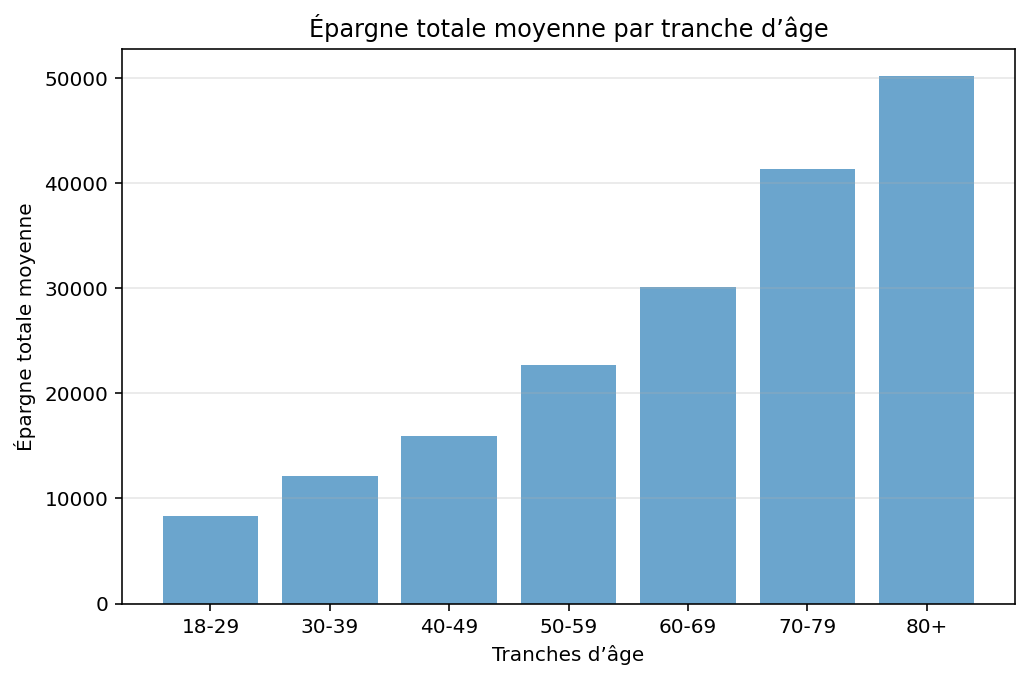
\includegraphics[width=0.5\textwidth]{images/py/epargneTotal_age.png}
    \caption{Histogramme de l'épargne totale selon l'âge}
\end{figure}

On observe une tendance claire : plus l'âge augmente, plus la moyenne d'épargne totale croît.  
Cela suggère un effet d'accumulation patrimoniale au fil du temps.

\subsubsection*{2. Histogramme de l'épargne financière par rapport à l'âge}
\begin{figure}[!h]
    \centering
    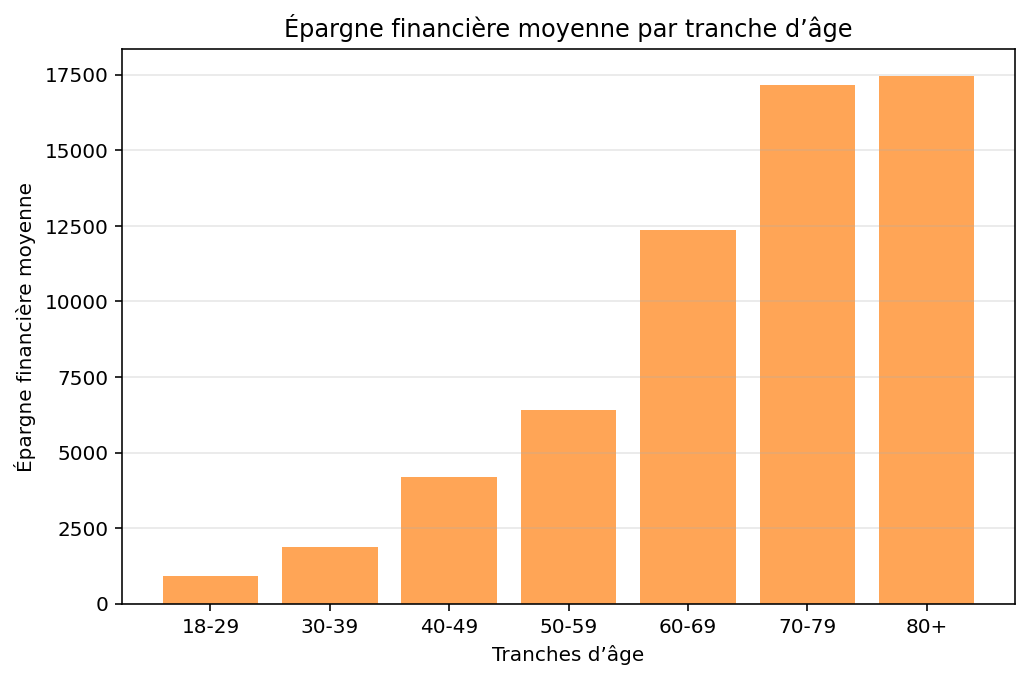
\includegraphics[width=0.5\textwidth]{images/py/eparge_fin_age.png}
    \caption{Histogramme de l'épargne financière selon l'âge}
\end{figure}

La même relation est visible que pour l'épargne totale : l'épargne financière progresse également avec l'âge, traduisant une capacité d'investissement plus forte chez les individus plus âgés.

\newpage\subsubsection*{3. Répartition de l'épargne totale par CSP}
\begin{figure}[h]
    \centering
    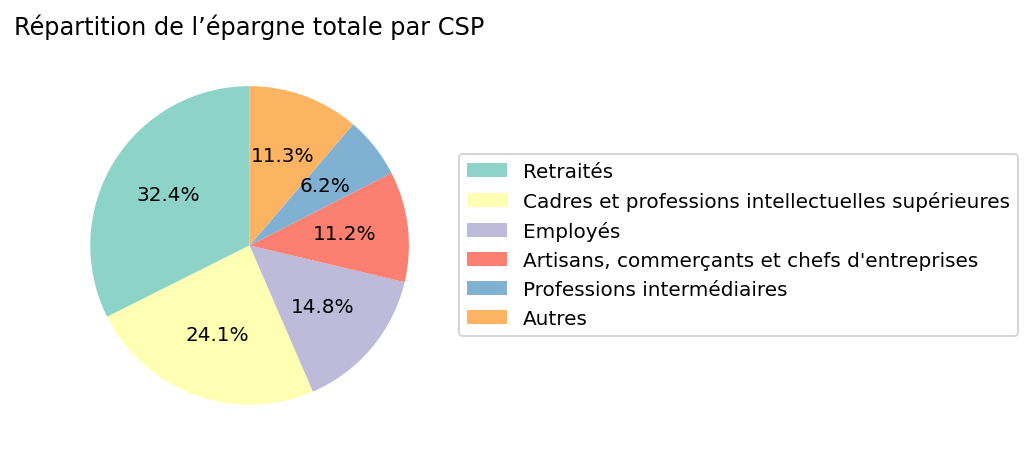
\includegraphics[width=0.6\textwidth]{images/py/CSP_epargne.png}
    \caption{Camembert de la répartition de l'épargne totale par CSP}
\end{figure}

La répartition montre que :  
- les \textbf{retraités} concentrent la part la plus importante (32,4\%),  
- suivis des \textbf{cadres et professions intellectuelles supérieures} (24,1\%),  
- puis des \textbf{employés} (14,8\%),  
- et des \textbf{artisans, commerçants et chefs d'entreprises} (11,2\%).  

Les autres catégories représentent des parts plus réduites.  
Cela confirme que les retraités, bénéficiant souvent de temps d’accumulation et de revenus stables, détiennent l'épargne la plus importante.

\subsubsection*{4. Répartition de l'épargne financière par CSP}
\begin{figure}[h]
    \centering
    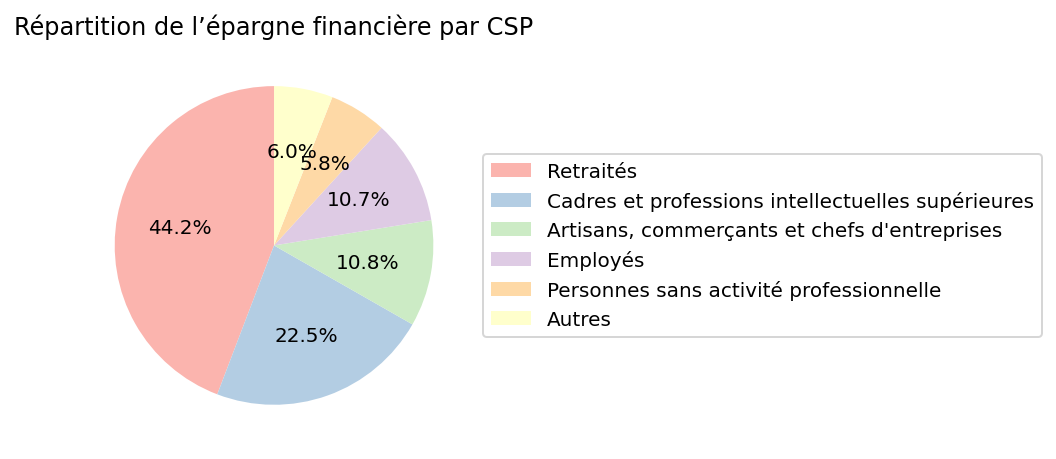
\includegraphics[width=0.6\textwidth]{images/py/csp_epargne_fin.png}
    \caption{Camembert de la répartition de l'épargne financière par CSP}
\end{figure}

La structure est encore plus marquée que pour l'épargne totale :  
- \textbf{44,2\% des retraités} concentrent à eux seuls près de la moitié de l'épargne financière,  
- suivis des \textbf{cadres et professions intellectuelles supérieures} (22,5\%).  

Les autres catégories (\textbf{artisans, employés, sans activité professionnelle}) se partagent le reste.  
Cette surreprésentation des retraités confirme leur rôle central dans l'épargne, probablement lié à une volonté de sécuriser le patrimoine.

\subsubsection*{5. Distribution des tranches d'épargne totale par marché}
\begin{figure}[!h]
    \centering
    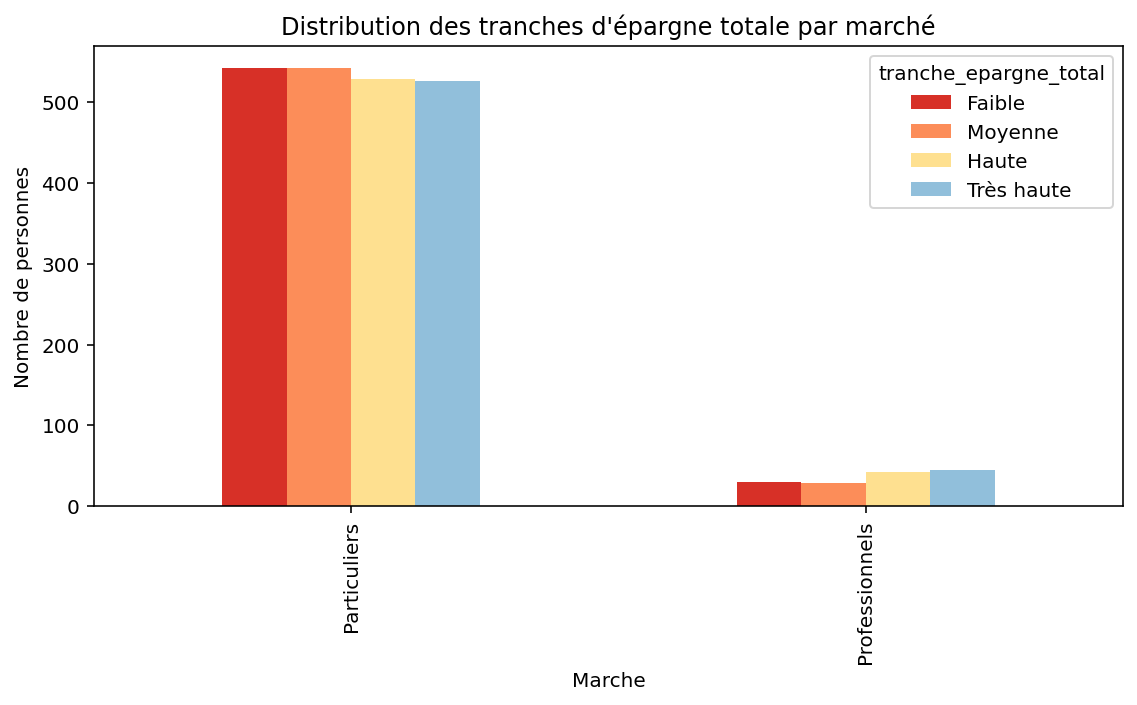
\includegraphics[width=0.7\textwidth]{images/py/epargne_total_marche.png}
    \caption{Histogramme des tranches d'épargne totale par marché}
\end{figure}

On constate une nette domination des particuliers, qui sont environ \textbf{cinq fois plus nombreux} que les professionnels.

\subsubsection*{6. Distribution des tranches d'épargne totale par type de client}
\begin{figure}[!h]
    \centering
    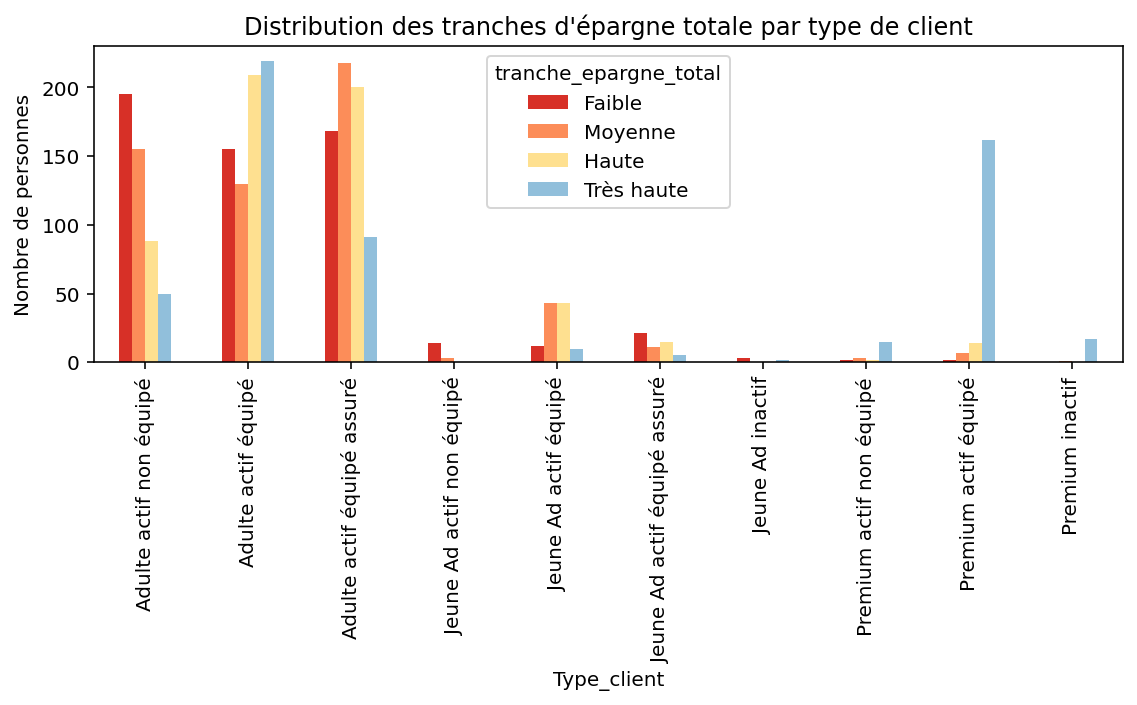
\includegraphics[width=0.7\textwidth]{images/py/epargne_total_typeClient.png}
    \caption{Histogramme des tranches d'épargne totale par type de client}
\end{figure}

L'analyse par type de client montre des contrastes importants :  
\begin{itemize}
    \item Les \textbf{adultes actifs non équipés} se concentrent surtout dans les tranches d’épargne faibles à moyennes
    \item Les \textbf{adultes actifs équipés}, en revanche, se distinguent par une forte présence dans les tranches hautes et très hautes, traduisant l'impact direct de l'équipement bancaire et assurantiel
    \item Les \textbf{adultes actifs équipés assurés} sont davantage répartis dans les niveaux faibles à moyens, ce qui suggère des profils plus hétérogènes
    \item Les \textbf{jeunes adultes actifs non équipés} disposent de très faibles niveaux d'épargne, quasiment inexistants dans les tranches supérieures
    \item Les \textbf{jeunes adultes actifs équipés (assurés ou non)} présentent une légère amélioration, mais restent globalement cantonnés aux tranches faibles à moyennes
    \item Les profils \textbf{premium} montrent un contraste très marqué : les \textbf{premium actifs équipés} et les \textbf{premium inactifs} concentrent quasi exclusivement leur épargne dans la tranche \textit{très haute}. Cela confirme leur statut patrimonial privilégié, fortement surreprésenté dans les épargnes les plus élevées
\end{itemize}

Ainsi, l'équipement bancaire et la catégorie premium apparaissent comme des facteurs discriminants majeurs pour expliquer le niveau d'épargne.

\subsection{Conclusion}

L'analyse exploratoire des données permet de dégager plusieurs enseignements clés :  

\begin{itemize}
    \item \textbf{Âge} : l'épargne (totale et financière) augmente régulièrement avec l'âge, confirmant un mécanisme d'accumulation patrimoniale.  
    \item \textbf{CSP} : les retraités dominent largement, suivis des cadres supérieurs, illustrant l'importance d'une carrière longue ou de revenus élevés dans la constitution d'un patrimoine.  
    \item \textbf{Marché} : les particuliers sont beaucoup plus nombreux, mais certains professionnels concentrent des montants d'épargne plus élevés.  
    \item \textbf{Type de client} : l'équipement joue un rôle central. Les adultes actifs équipés apparaissent comme les plus solides en termes d'épargne, tandis que les jeunes actifs non équipés restent vulnérables. Enfin, les profils premium sont quasi exclusivement positionnés dans les niveaux d'épargne les plus élevés, marquant une polarisation très forte.  
\end{itemize}

En résumé, l'âge, le statut socio-professionnel, l'équipement bancaire et l'appartenance à la catégorie premium constituent les principaux facteurs explicatifs de l'épargne.  
Ces résultats offrent une base précieuse pour la mise en place d'un modèle de prédiction visant à anticiper le potentiel d'épargne d'un individu en fonction de ses caractéristiques.

\end{document}